\section{Introduzione}
Durante la prima iterazione sono state identificate le componenti dal modello dei casi d'uso, 
applicando le euristiche di early design: viene perfezionata la specifica dei componenti 
progettati durante l'iterazione 0 al fine di da definire meglio l'architettura software. 
È stato costruito lo scheletro dell'applicazione tramite la specifica delle differenti classi 
popolate nelle seguenti iterazioni.

Inizialmente, durante lo sviluppo dell'iterazione 0, il sistema nella sua totalità è stato 
visualizzato come una unica componente e sono stati 
introdotti gli attori, ognuno dei quali definito come un'entità esterna. In seguito sono stati 
sviluppati tutti i casi d'uso che riassumono il funzionamento del sistema, i quali vengono, 
nella prima iterazione, raccolti e raggruppati secondo un preciso criterio e affinità. 

Vengono inoltre introdotti componenti e sottocomponenti di controllo di ciascun gruppo, o 
alternativamente componenti di dati; per ognuno di essi nascono parallelamente le classi 
candidate e le relazioni che le legano. 

Per ogni caso d'uso che ha una interazione diretta con un attore esterno viene introdotta 
un'interfaccia per le operazioni visibili esternamente, ovvero le API, offerte o richieste 
dal componente o sottocomponente corrispondente, in base alla direzione dell'interazione. 

Ogni variabile input/output da un attore, specificata nella descrizione di un caso d'uso, 
definisce un parametro di input/di ritorno dell'operazione dell'interfaccia corrispondente. 

Viene quindi scomposto il sistema in sottosistemi e componenti, applicando pattern e 
stili architetturali, per poi distribuire le componenti su nodi computazionali basati su 
uno sviluppo fisico del sistema.


E' necessario specificare che l'architettura di Django si basa sul design pattern \textbf{MVC}, acronimo di Model View 
Controller. Lo scopo di questa scelta di design è la suddivisione della logica in 
tre parti fondamentali favorendo modularità, sviluppo collaborativo e riutilizzo del 
codice oltre a rendere l'applicazione più flessibile e scalabile.
    
Django interpreta il pattern MVC a modo suo, in modo tale che il Controller risulti in 
realtà il framework in sé, le View non scelgano come i dati vadano mostrati bensì quali 
dati mostrare e il come mostrarli viene in realtà deciso nei Template.

Siccome la parte del Controller è gestita dal framework e la View è rappresentata dai Template, Django 
utilizza un framework MTV, ovvero \textbf{Model Template View}.
    
\begin{comment}
Per prima cosa quando viene effettuata una richiesta HTTP essa viene confrontata con gli URL, 
che sono una “mappa” delle risorse disponibili. La richiesta viene quindi inoltrata alla View 
che la gestisce producendo una risposta HTTP della cui formattazione si occuperanno i template, 
mentre il Model fornirà la logica per accedere ai dati e convertirli in tabelle nel database. 

\end{comment}
   
\begin{itemize}
    \item \textbf{M - Model:} “data access layer” - Definisce la struttura delle entità (le classi) del nostro sito, tradotte 
    poi in tabelle nel database.
    \item \textbf{T - Template:} “presentation layer” - Descrive come i dati vadano mostrati nelle pagine web.
    \item \textbf{V - View:} “business logic layer” - Gestisce le richieste e le risposte HTTP, dispone della 
    logica per sapere a quali dati accedere tramite i model e delega la formattazione della risposa ai template, contenendo quindi i metodi. 
\end{itemize}
    
    
\newpage

\section{Casi d'uso}
I casi d'uso vengono raggruppati in tre macro categorie in base a un criterio di affinità:
i primi sono relativi all'autenticazione dell'utente, i secondi sono relativi a tutto
ciò che riguarda l'ambito musicale, ed infine quelli relativi all'account personale e lato social. 
Di seguito un elenco dettagliato dei casi d'uso suddivisi come anticipato.

\subsection{Autenticazione}
    \begin{itemize}
        \item \textbf{UC1:} Sign up 
        \item \textbf{UC2:} Sign in
        \item \textbf{UC3:} Sign out 
    \end{itemize}


\subsection{Musica}
\begin{itemize}
    \item \textbf{Brano:} in questa sezione rientrano tutti i casi d'uso relativi ai brani.
    \begin{itemize}
        \item \textbf{UC4:} Cerca brano
        \item \textbf{UC5:} Cerca album
        \item \textbf{UC6:} Cerca Artista
        \item \textbf{UC7:} Scarica brano
        \item \textbf{UC8:} Like al brano
        \item \textbf{UC19:} ``Discover'' 
    \end{itemize} 
    
    \item \textbf{Playlist:} in questa sezione rientrano tutti i casi d'uso relativi alla creazione e gestione delle playlist.
    \begin{itemize}
        \item \textbf{UC9:} Aggiungi brano a playlist
        \item \textbf{UC15:} Visualizza playlist 
        \item \textbf{UC16:} Crea nuova playlist 
        \item \textbf{UC17:} Elimina playlist
        \item \textbf{UC18:} Modifica playlist
    \end{itemize}
    
    \item \textbf{Artista:} in questa sezione rientrano tutti i casi d'uso relativi alla gestione del profilo artista.
    \begin{itemize}
        \item  \textbf{UC20:} Crea pagina artista 
        \item  \textbf{UC21:} Visualizza pagina artista 
        \item  \textbf{UC22:} Aggiungi brano 
        \item  \textbf{UC23:} Aggiungi album 
        \item  \textbf{UC24:} Personalizza pagina artista 
        \item  \textbf{UC25:} Consulta anagrafica
    \end{itemize} 
\end{itemize}

\subsection{Account}
\begin{itemize}
    \item \textbf{Personale:} in questa sezione rientrano tutti i casi d'uso relativi alla gestione delle informazioni nel proprio profilo personale.
    \begin{itemize}
        \item \textbf{UC12:} Visualizza informazioni profilo 
        \item \textbf{UC13:} Modifica profilo 
        \item \textbf{UC14:} Elimina profilo 
    \end{itemize}
    
    \item \textbf{Amici:} in questa sezione rientrano tutti i casi d'uso relativi alla parte social.
    \begin{itemize}
        \item \textbf{UC10:} Cerca Utente 
        \item \textbf{UC11:} Aggiungi Utente 
    \end{itemize}
\end{itemize}






\newpage

\section{UML Data Class Diagram}
Il Class Diagram in UML permette di descrivere il sistema 
visualizzando i diversi tipi di oggetti all'interno di esso e le relazioni 
statiche che esistono fra loro: sono descritte in maniera più approfondita 
le tre componenti già precedentemente analizzate, ovvero Account, Musica, 
Autenticazione e Discover.
In questo caso viene rappresentato in unico diagramma il Data Class Diagram, 
il quale descrive le classi che compongono la struttura dell'applicazione e le
le entità presenti al suo interno, e il Package/IF Diagram, quindi sono stati
inserite le funzioni implementate. 
nel sistema.
\begin{figure}[H]
    \centering
    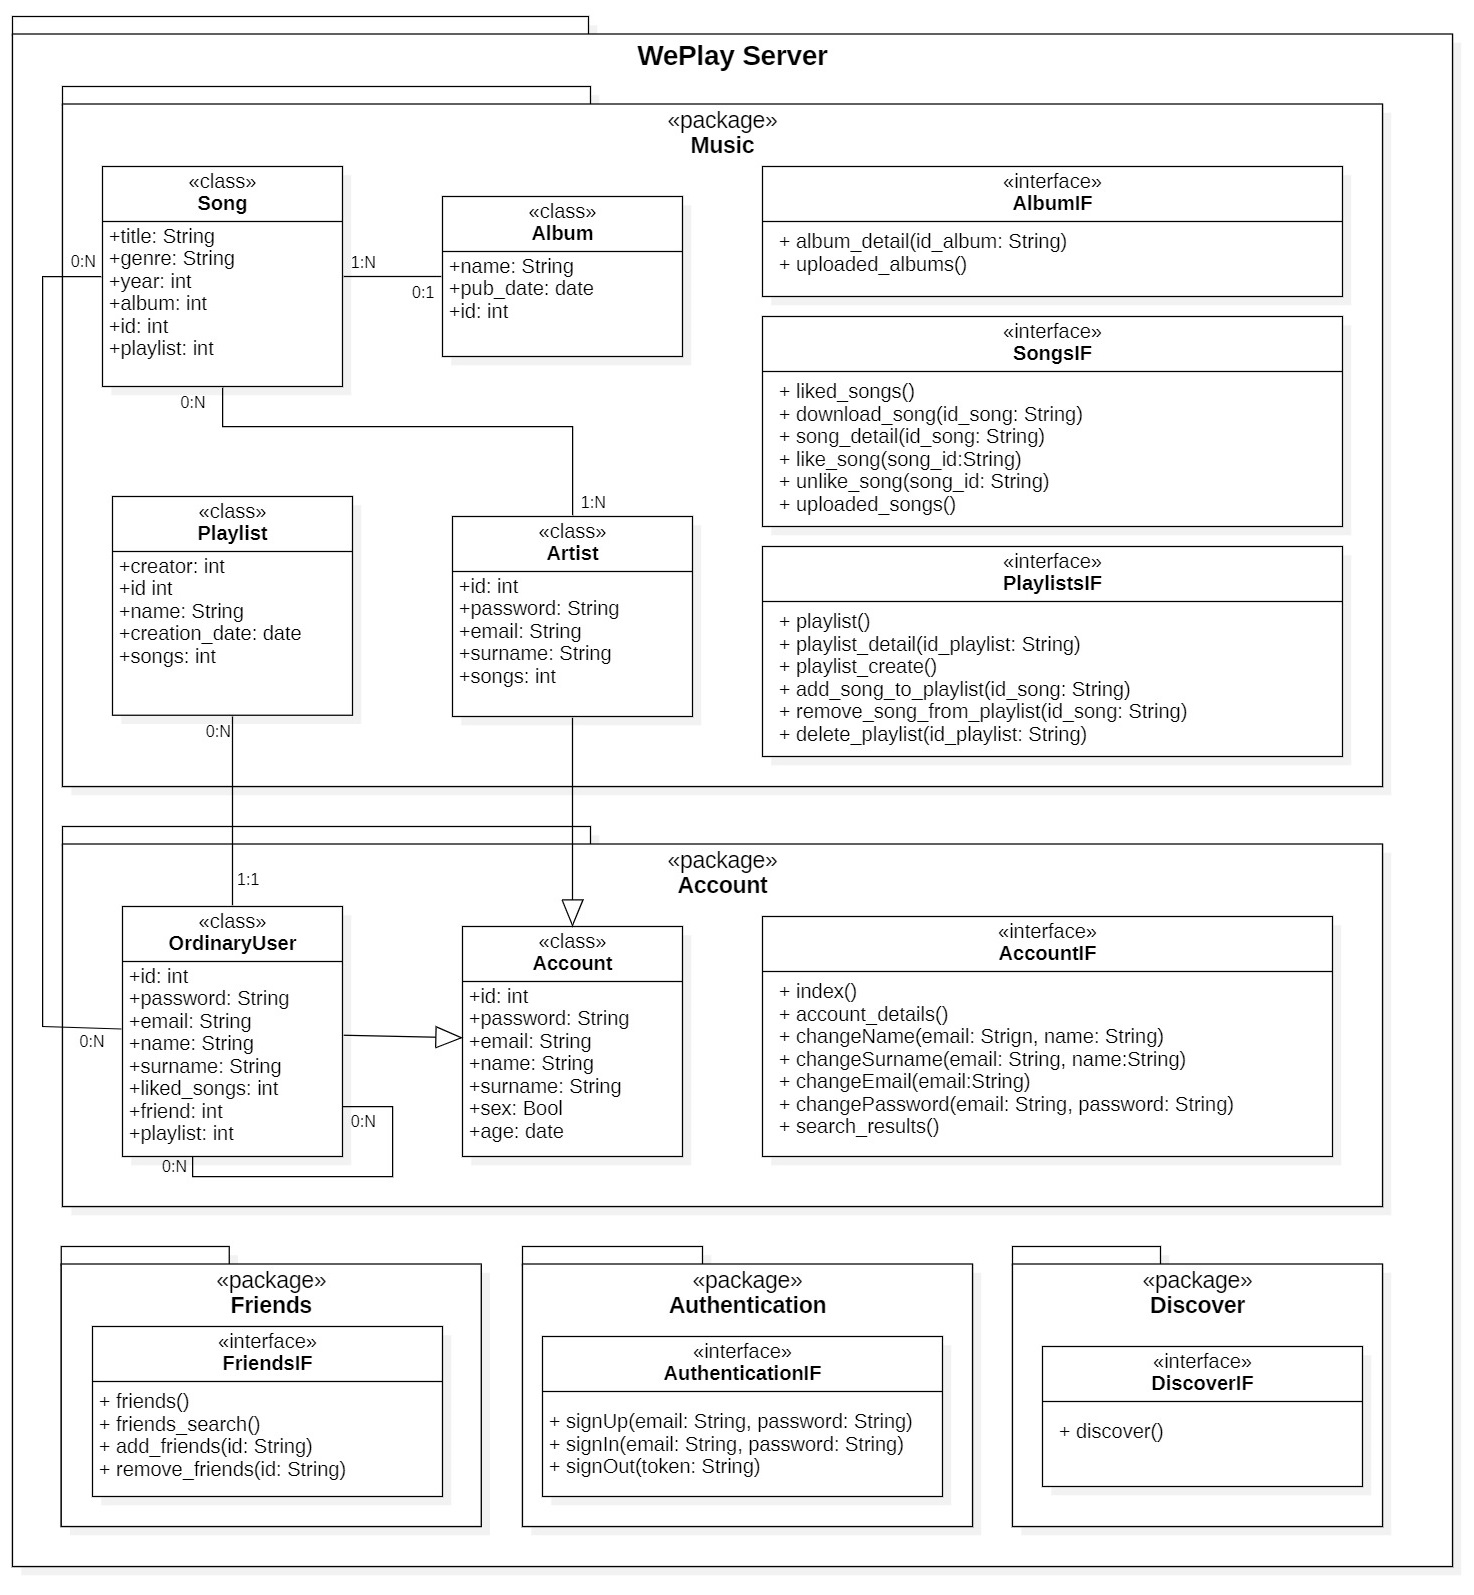
\includegraphics[scale=0.4]{images/ClassDiagram_ver6.jpg}
    \caption{UML Class Diagram}
    \label{fig-uml-class-diag}
\end{figure}
\newpage

\section{UML Component Diagram}
Il Component Diagram in UML ha come obiettivo quello di mostrare la struttura
del sistema software, descrivendo i singoli componenti, le relative interfacce 
e le dipendenze. 

\vspace{2cm}
\subsection{Black Box - Top level}
La rappresentazione black box del sistema è stata gestita partendo da una
una componente centrale, il server del sistema, alla quale si collegano il database e la parte front-end.
Le componenti principali sono: Account, Authentication, Music (che include Brani, Playlist, Album),
Discover e Friends.
\begin{figure}[H]
    \centering
    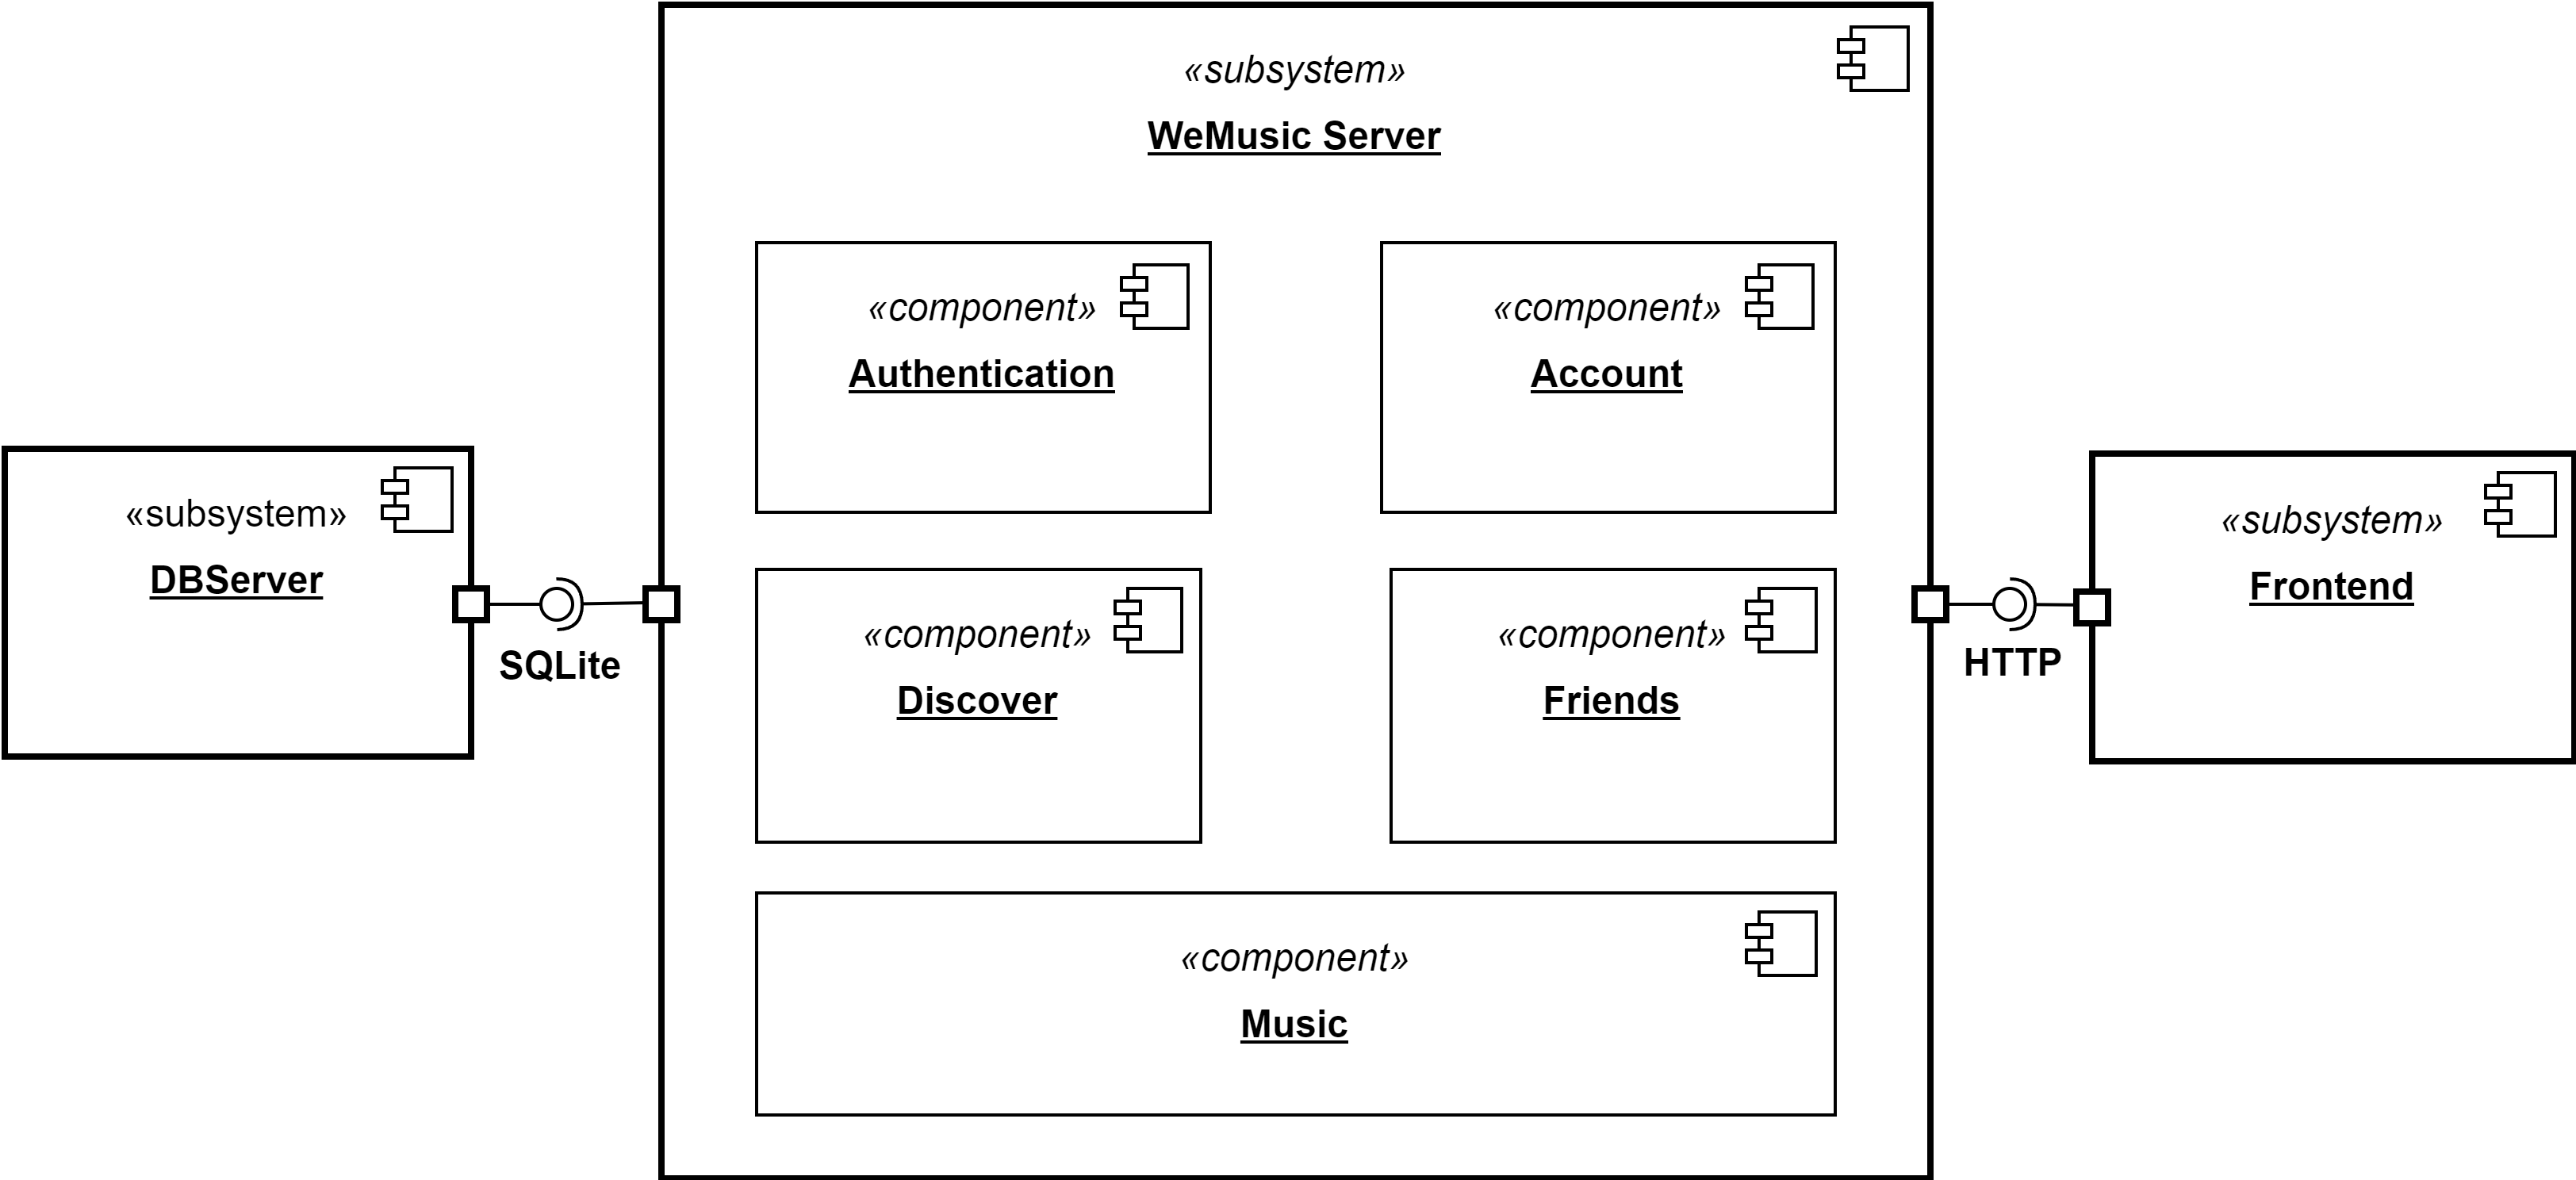
\includegraphics[scale=0.65]{component_diagram_ver4_1.png}
    \caption{UML Component Diagram}
    \label{fig-uml-component-diag_1}
\end{figure}

\newpage
\subsection{White Box - Top level}
La rappresentazione white box del sistema rappresenta anche le componenti
interne e le interfacce tramite le quali comunicano tra loro.

\begin{figure}[H]
    \centering
    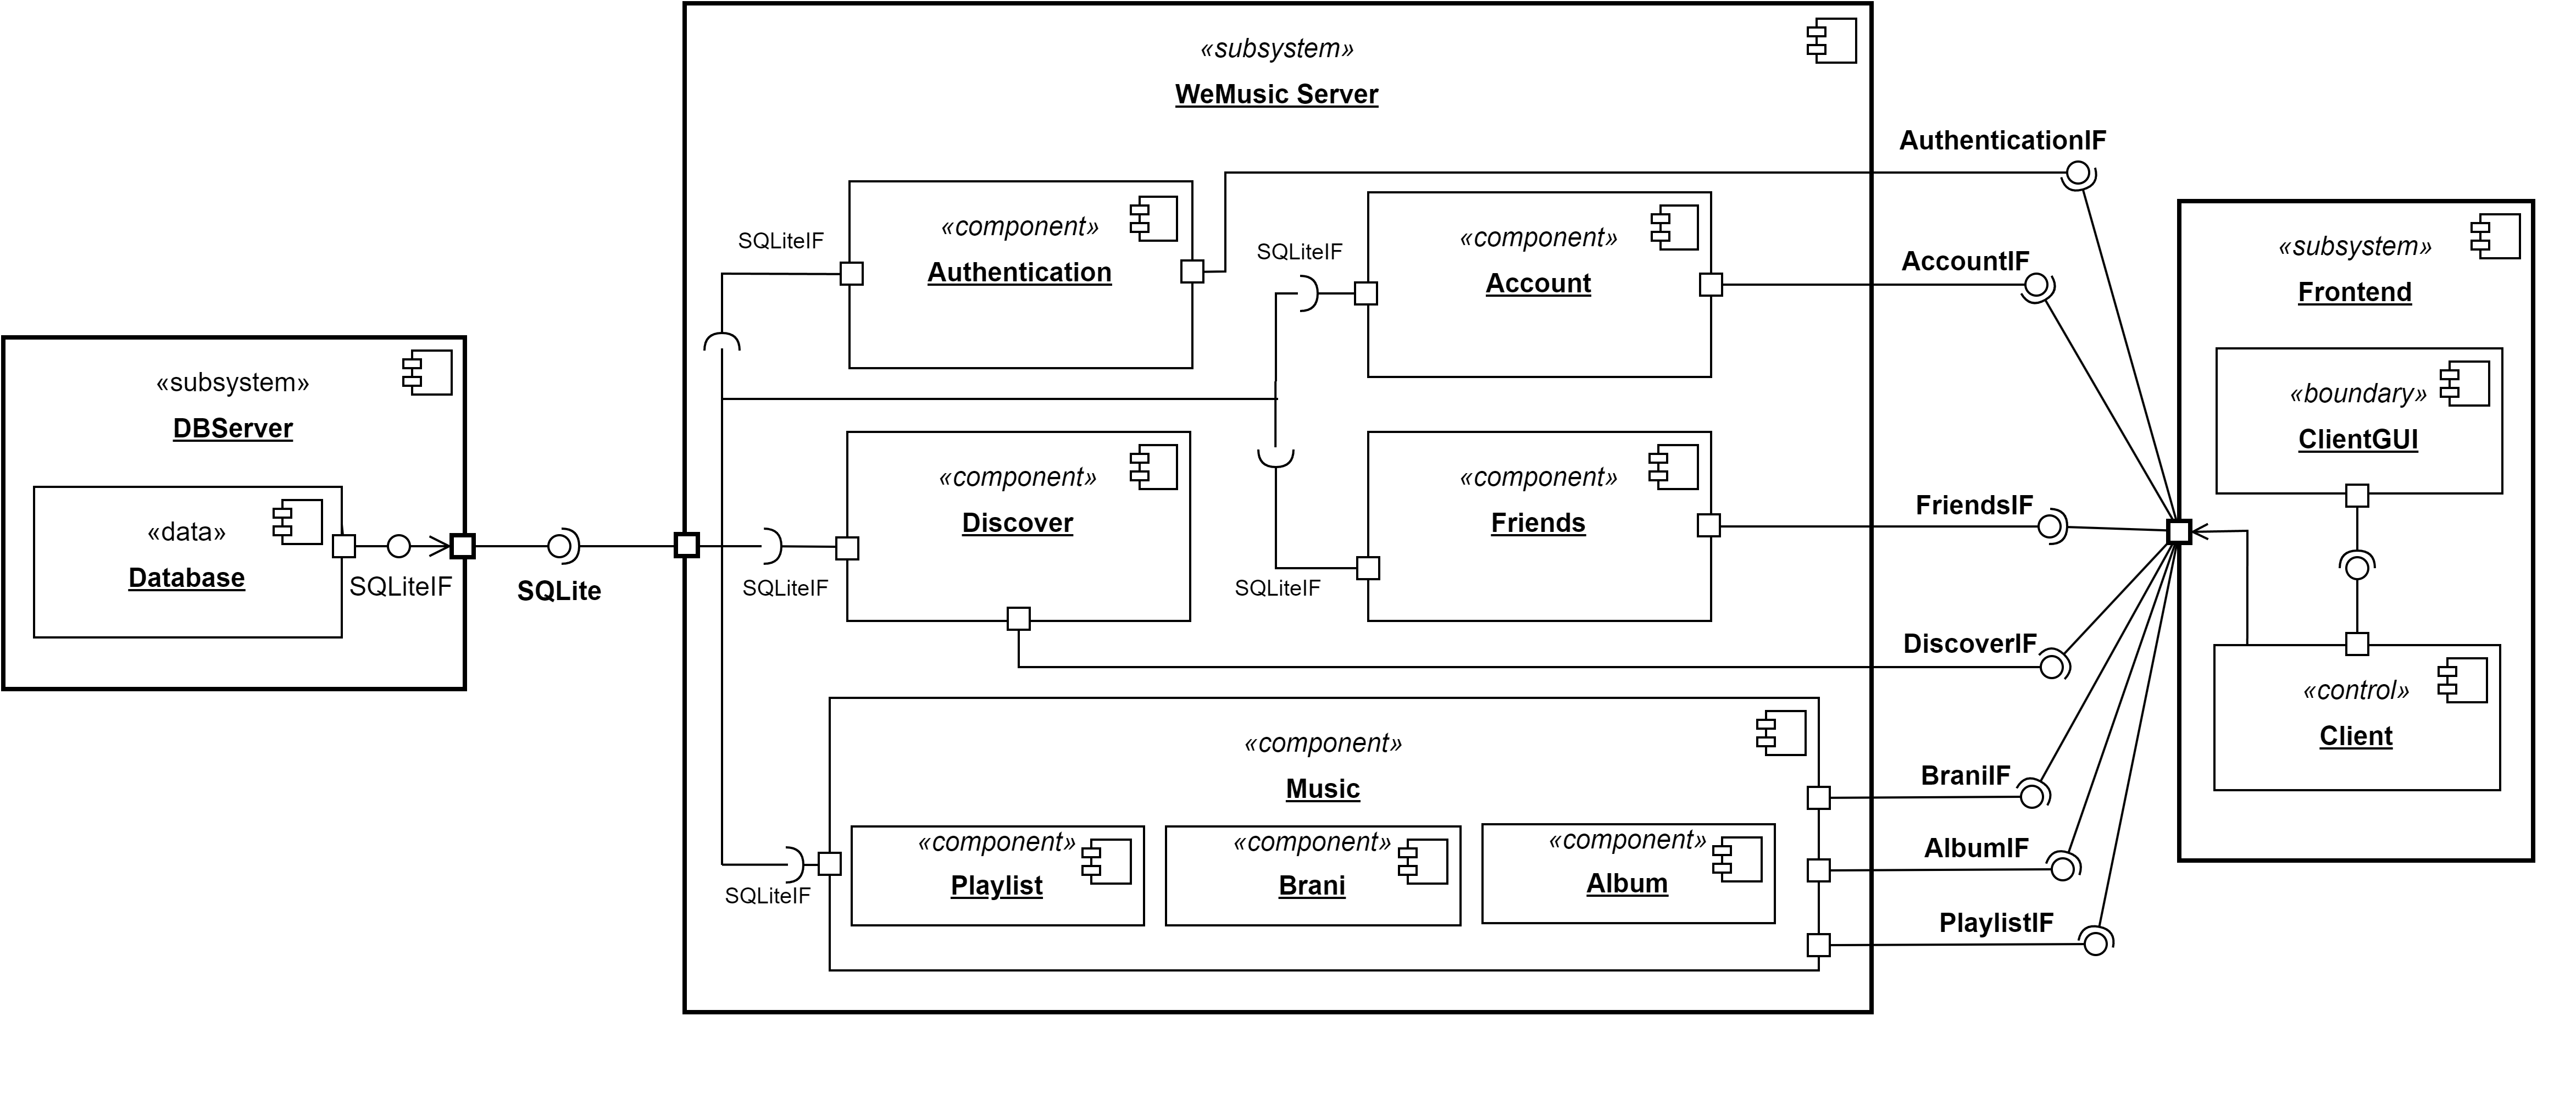
\includegraphics[scale=0.13]{component_diagram_ver4_2.png}
    \caption{UML Component Diagram}
    \label{fig-uml-component-diag_2}
\end{figure}

